\documentclass[tikz,border=8pt]{standalone}
\usepackage[dvipsnames]{xcolor}
\usetikzlibrary{shapes.geometric,arrows.meta,positioning,fit,backgrounds,calc,decorations.pathreplacing}

\begin{document}
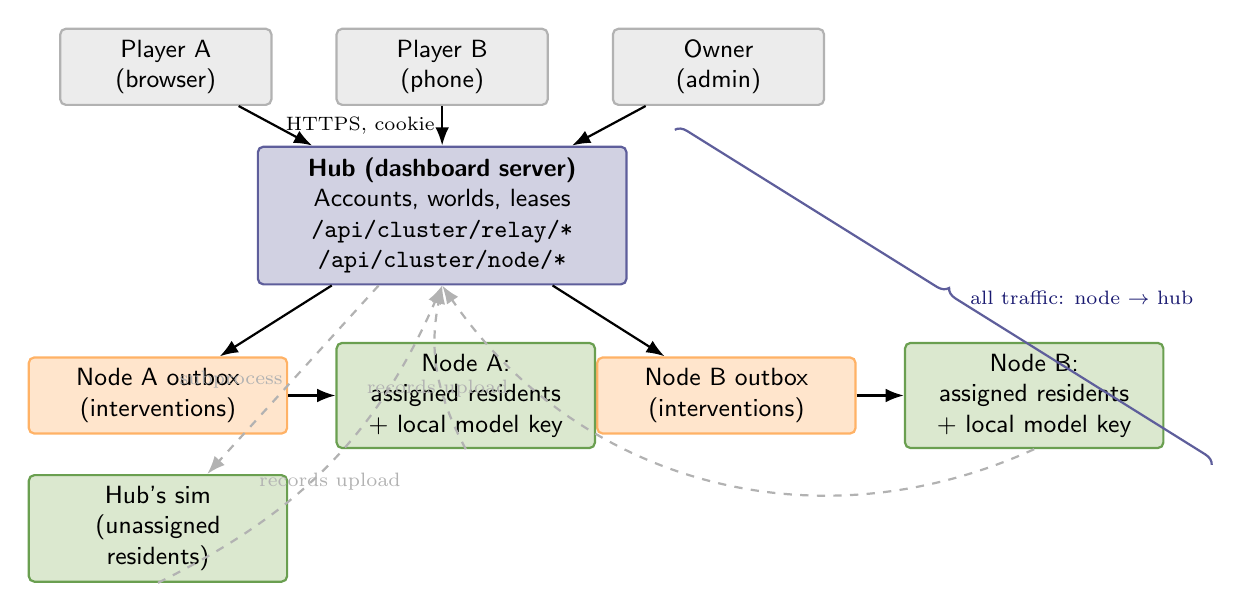
\begin{tikzpicture}[
  font=\sffamily\small,
  box/.style={rectangle, draw, thick, rounded corners=2pt, align=center, minimum height=0.9cm, inner sep=4pt},
  hub/.style={box, fill=MidnightBlue!20, draw=MidnightBlue!70, text width=4.4cm},
  node/.style={box, fill=OliveGreen!15, draw=OliveGreen!70, text width=3.0cm},
  browser/.style={box, fill=gray!15, draw=gray!60, text width=2.4cm},
  outbox/.style={box, fill=orange!20, draw=orange!60, text width=3.0cm},
  relay/.style={box, fill=Purple!15, draw=Purple!60, text width=3.0cm},
  ar/.style={-Latex, thick},
  >={Stealth[length=2.5mm]}
]

% Browsers (top)
\node[browser] (b1) at (0,0) {Player A\\(browser)};
\node[browser, right=0.8cm of b1] (b2) {Player B\\(phone)};
\node[browser, right=0.8cm of b2] (b3) {Owner\\(admin)};

% Hub (center)
\node[hub, below=1.0cm of $(b1)!0.5!(b3)$] (hub) {%
  \textbf{Hub (dashboard server)}\\
  Accounts, worlds, leases\\
  \texttt{/api/cluster/relay/*}\\
  \texttt{/api/cluster/node/*}};

% Per-node outbox (between hub and nodes)
\node[outbox, below left=0.9cm and -0.4cm of hub] (ob1) {%
  Node A outbox\\(interventions)};
\node[outbox, below right=0.9cm and -0.4cm of hub] (ob2) {%
  Node B outbox\\(interventions)};

% Hub's own sim (left below)
\node[node, below=0.5cm of ob1] (simh) {%
  Hub's sim\\(unassigned residents)};

% Two external nodes
\node[node, right=0.6cm of ob1] (n1) {%
  Node A:\\
  assigned residents\\
  + local model key};
\node[node, right=0.6cm of ob2] (n2) {%
  Node B:\\
  assigned residents\\
  + local model key};

% Edges
\draw[ar] (b1) -- node[right, font=\scriptsize]{HTTPS, cookie} (hub);
\draw[ar] (b2) -- (hub);
\draw[ar] (b3) -- (hub);
\draw[ar] (hub) -- (ob1);
\draw[ar] (hub) -- (ob2);
\draw[ar] (ob1) -- (n1);
\draw[ar] (ob2) -- (n2);
\draw[ar, dashed, gray!60] (hub) -- node[left, font=\scriptsize]{subprocess} (simh);
\draw[ar, dashed, gray!60] (simh.south) to[bend right=20] node[below, font=\scriptsize]{records upload} (hub.south);
\draw[ar, dashed, gray!60] (n1.south) to[bend left=20] node[below, font=\scriptsize]{records upload} (hub.south);
\draw[ar, dashed, gray!60] (n2.south) to[bend left=40] (hub.south);

% Bracket on the right: "all traffic node → hub"
\draw[decorate, decoration={brace, amplitude=4pt, mirror}, thick, MidnightBlue!70]
  ($(n2.south east)+(0.6cm,-0.2cm)$) -- ($(hub.north east)+(0.6cm,0.2cm)$)
  node[midway, right=6pt, font=\scriptsize, text=MidnightBlue]{%
    all traffic: node $\rightarrow$ hub};

\end{tikzpicture}
\end{document}
